\documentclass[12pt, a4paper]{article}
\PassOptionsToPackage{sharp}{prettytex/boxes}
\usepackage{prettytex/base}

\setlength{\topmargin}{0.0in}
\setlength{\oddsidemargin}{0.33in}
\setlength{\textheight}{9.0in}
\setlength{\textwidth}{6.0in}
\renewcommand{\baselinestretch}{1.25}

\usepackage{prettytex/math}
\usepackage[nameinlink]{cleveref}
\usepackage[cleveref]{prettytex/math-theorems}
\usepackage{prettytex/mathematicians}
\usepackage{prettytex/gfx}
\usepackage{prettytex/code}
\usepackage{prettytex/pseudo}
\usepackage{prettytex/thesis}

\setlength{\headheight}{19.53pt}
\setlength{\headsep}{1.8em}
\setlength{\belowcaptionskip}{-12pt}
\addbibresource{sources.bib}

\newcommand{\topictitle}{Solving PDEs using Spectral Methods in the Chebyshev basis \\ \large by example of the Heat Equation}
\newcommand{\candidatenumber}{12345}
\newcommand{\course}{Approximation of Functions}
\newcommand{\tschebfun}{TschebFun}
\newcommand{\heatfun}{HeatFun}

\title{\topictitle}
\author{Candidate \candidatenumber}
\date{\today}

\setminted{fontsize=\footnotesize}
\AfterEndEnvironment{minted}{\vspace*{-0.8cm}}

\tikzexternalize[prefix=tikz/]

% Outline:
% ✅ Setting: define heat equation PDE problem (with BCs), explain series in x direction
% ✅ Introduce Chebyshev polynomials (relation of x, z and theta)
% ✅ Prove recurrence relation
% ✅ Prove orthogonality
% ✅ - Using transformation to theta
% ✅ - cite Cauchy integral for Laurent series
% ✅ Define Lipschitz
% ✅ Define Function Space in Cheb Basis
% ✅ Introduce Cheb series
% ✅ Algorithm one: interpolantThrough()
% ✅ - Method one: Rectangular integral approx. rule
% ✅ - Method two: DCT
% ✅ - Method three: Barycentric formula
% ✅ Algorithm two: evaluateOn()
% ✅ Numerics: Define Forward Euler
% ✅ Algorithm three: differentiation of a Cheb series
% - Method one: via DCT
% - Method two: via recursion formula
% ✅ - Method three: via finite differences and repeated interpolantThrough()
% ✅ Final application: interpolantThrough(), u_1 = alpha * dt * diff(diff(u_0)), evaluateOn()
% ✅ Results
% TODO: chebfun supports solving using both the spectral method as well as time-stepping methods [TAD14 - ChebFun guide].
% TODO: D_N matrix is (N+1) x (N+1) or N x (N+1)??

\begin{document}
  \pagestyle{plain}
  \begin{center}
    \vspace*{-2.5cm}
    \Large \topictitle \\
    \vspace{.3cm}

    \normalsize Special Topic on \textcolor{themecolor3}{\textsc{\course}}\\
    \normalsize Candidate Number: \textcolor{themecolor3}{\candidatenumber}
    \vspace{.3cm}
  \end{center}

  \begin{abstract}
    This work shall attempt to numerically solve the heat equation $u_t = \alpha u_{xx}$ with Dirichlet boundary conditions over the domain $[-1, 1] \times [0, T]$ by representing the spatial component as a \textit{chebfun} (Chebyshev series) and moving on in time by the Forward Euler numerical scheme.
    \vspace*{0.2cm}

    \noindent
    \textbf{Our Goal:}
    Numerically obtain the solution $u(x, T)$ of
    \vspace*{-0.2cm}
    $$\begin{cases}
        \frac{\partial u}{\partial t} = \alpha \frac{\partial^2 u}{\partial x^2} \quad & u: [-1, 1] \times [0, T] \mapsto \R,\, T \in \R^+,\; \alpha \in \R^+         \\
        u(x_j, 0) = u_0(x_j) \quad                                                     & \forall x_j \in \tilde{X}_N,\; N \in \N,\, N > 1, \; u_0: [-1, 1] \mapsto \R \\
        u(b, t) = u_0(b)                                                               & \forall b \in \{-1, 1\},\; \forall t \in (0, T] \,.
      \end{cases}$$
    \vspace*{0.05cm}

    The implementation, centered around what we will refer to as \textbf{\textcolor{themecolor3}{TschebFun}}, including three major algorithms \texttt{\textcolor{themecolor3}{TschebFun}::\textcolor{themecolor2}{interpolantThrough}()}, \texttt{\textcolor{themecolor3}{TschebFun}::\textcolor{themecolor2}{evaluateOn}()} and \texttt{\textcolor{themecolor3}{TschebFun}::\textcolor{themecolor2}{derivative}()}, is done manually in C++, extended to work as a Python module and for demonstration, even features a high-level graphical interface to play with.
    Finally, we will compare the numerical results with the output of \textit{Chebfun}'s high-level \texttt{pde15s()}.
  \end{abstract}

  \begin{figure}[H]
    \centering
    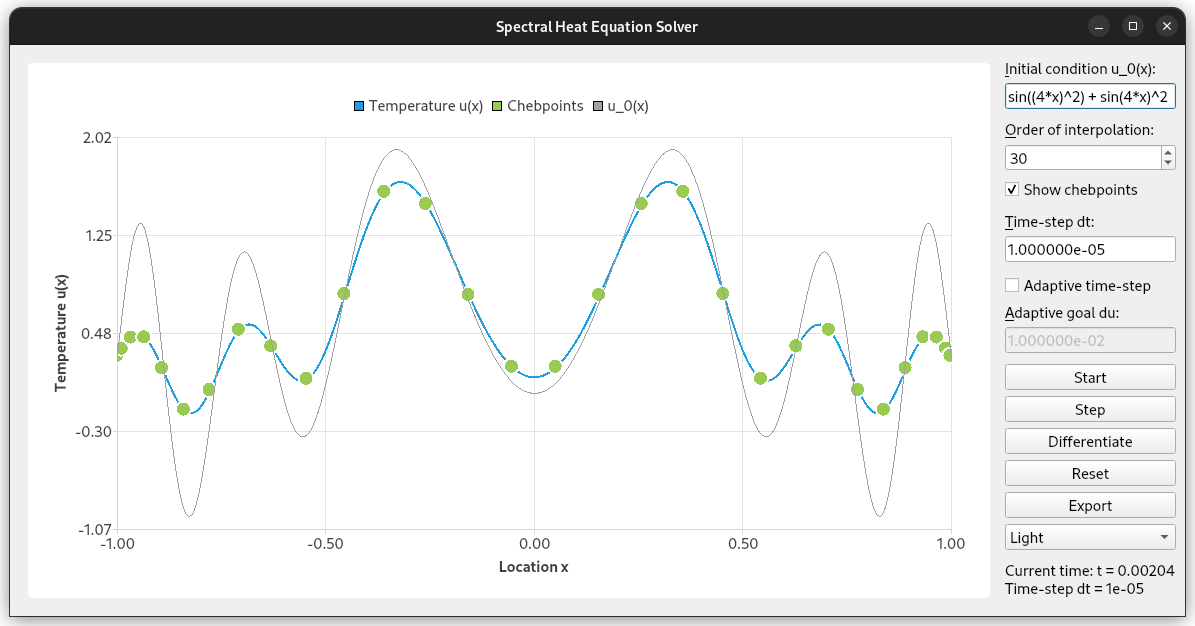
\includegraphics[width=\linewidth]{figures/screenshot.png}
    \caption{Screenshot of the graphical user interface. After entering an initial expression $u_0(x)$, depicted in grey, the simulation will run upon pressing 'Start'. The solution at time $t$, depicted in blue, is represented as a Chebyshev series of degree 29.}
  \end{figure}

  \pagebreak
  \pagestyle{normal}

  % \tableofcontents
  % \pagebreak

  \section{Motivation}
  Partial differential equations are notoriously hard to solve. One more possible approach to make way in this important class of problems is by the technique of spectral methods, incidentally closely related to finite element methods.
  The key idea is to perform the problem solution by representation of the occurring functions in a certain basis.
  For non-periodic problem settings, \textsc{Chebyshev} series are a fantastic choice.

  % \subsection{The Heat Equation and Our Method}
  Classical approaches to solving the heat equation are:
  \begin{itemize}
    \item Using the separation Ansatz
          $$u(x, t) = \underline{X}(x) \underline{T}(t), \quad \underline{X}: [-1, 1] \mapsto \R, \quad \underline{T}: [0, T] \mapsto \R$$
          one obtains a first- and second-order constant-coefficient ordinary differential equation in $t$ and $x$, respectively. Of course, this is only applicable to suitable initial conditions.

    \item By Fourier-analysis: Similar to our approach below, or maybe even simpler: differentiation simply multiplies the Fourier coefficients by $\i k$, with $k$ the wave number. This is a spectral method!

    \item Numerically, a finite difference scheme such as
          $$\frac{U_{j}^{(n+1)} - U_{j}^{(n)}}{\Delta t} = \alpha \frac{U_{j+1}^{(n)} - 2 U_{j}^{(n)} + U_{j-1}^{(n)}}{(\Delta x)^2}$$ can be used to solve the problem.
  \end{itemize}

  Our method focusses on a combination of a spectral method (for the spatial component) and finite difference approximation (for the temporal component).

  The first step is to interpolate through the initial data $\{(x_j, u_0(x_j)) \;|\; x_j \in X_N\}$, iteratively modify the resulting coefficients according to the partial differential equation and finally obtain a series representation of the solution after time $T$.

  \pagebreak
  \section{Chebyshev Interpolation}
  Let $\N$ denote the nonnegative integers, so $0 \in \N$.

  \begin{definition}{Chebyshev polynomial}{chebpoly}
    Chebyshev\footnote{named after Pafnuty Lvovich \textsc{Chebyshev}, alternatively transliterated as Tchebycheff, Tchebyshev (French) or \textsc{Tschebyschow} (German)} polynomials $T_k: \R \mapsto \R$ are functions satisfying
    \begin{align*}
      T_k(x) = T_k(\cos \theta) := \cos(k \theta) = \frac{1}{2} (z^k + z^{-k}) \\
      z := \e^{i \theta},\quad x := \Re(z) = \cos(\theta) = \frac{1}{2}(z + z^{-1})
    \end{align*}
    for degree $k \in \N$. Then, $T_0(x) = 1$, $T_1(x) = x$, $T_2(x) = 2x^2-1$, and so on.
  \end{definition}

  The above relations between $x$, $z$ and $\theta$ reveal fundamental connections between three famous basis sets: \textsc{Chebyshev}, \textsc{Laurent} and \textsc{Fourier}.

  There is a handy method of explicitly writing out the Chebyshev polynomials in $x$, namely by a three-step recursion with $T_0(x) = \cos(0) = 1$ and $T_1(x) = \cos(\theta) = x$.

  \begin{theorem}{Chebyshev recursion formula}{chebrecursion}
    The Chebyshev polyomials satisfy the three-term recurrence relation $$T_{k+1}(x) = 2x T_k(x) - T_{k-1}(x) \,.$$
  \end{theorem}
  \begin{proof}
    For $k > 1$, we have
    \begin{align*}
      2x T_k(x) - T_{k-1}(x) & = 2x \frac{1}{2} (z^k + z^{-k}) - \frac{1}{2} (z^{k-1} + z^{-(k-1)})                       \\
                             & = 2 \frac{1}{2}(z + z^{-1}) \frac{1}{2}(z^k + z^{-k}) - \frac{1}{2} (z^{k-1} + z^{-k+1})   \\
                             & = \frac{1}{2} (z^{k+1} + z^{k-1} + z^{-k+1} + z^{-k-1}) - \frac{1}{2} (z^{k-1} + z^{-k+1}) \\
                             & = \frac{1}{2} (z^{k+1} + z^{-(k+1)}) = T_{k+1}(x)
    \end{align*}
  \end{proof}

  \subsection{An Orthogonal Basis}
  The Chebyshev polynomials also satisfy an \emph{orthogonality relation},
  $$\langle T_m, T_n \rangle := \int_{-1}^1 T_m(x) T_n(x) \frac{1}{\sqrt{1-x^2}} \ddx = \int_{\pi}^{0} \cos(m \theta) \cos(n \theta) \frac{-\sin(\theta)}{\sqrt{1-\cos^2(\theta)}} \dd\theta \,,$$
  which becomes, with the fitting substitution $x = \cos(\theta)$ and $\ddx = -\sin(\theta) \dd\theta$,
  \begin{align*}
    \langle T_m, T_n \rangle & = \int_0^\pi T_m(\cos \theta) T_n(\cos \theta) \frac{\sin \theta}{\sin \theta}\dd\theta = \int_0^\pi \cos(m \theta) \cos(n \theta) \dd\theta                            \\
                             & = \frac{1}{2} \int_0^\pi \big(\underbrace{\cos((m+n) \theta)}_{=\cos(2m\theta) \text{ for } m=n} + \underbrace{\cos((m-n) \theta)}_{=1 \text{ for } m=n}\big) \dd\theta
  \end{align*}
  along with the knowledge that $\int_0^\pi \cos(k \theta) \dd\theta = k^{-1} \left[\sin(k\theta)\right]_0^\pi = 0$ for $k \in \Z \backslash \{0\}$,
  $$\langle T_m, T_n \rangle = \int_0^\pi T_m(\cos \theta) T_n(\cos \theta) \dd\theta = \begin{cases}
      0     & \text{ for } m \neq n     \\
      \pi/2 & \text{ for } m = n \neq 0 \\
      \pi   & \text{ for } m = n = 0
    \end{cases}$$
  which can be effectively utilised to define a function space $(\mathbb{T}, +, \cdot)$ in the \emph{orthogonal} basis of Chebyshev polynomials $\mathcal{T} := \{T_k\}_{k \in \N}$.
  Note that the operation $\langle \cdot, \cdot \rangle$ satisfies all axioms of an authentic inner product (linearity, etc.) over a function space due to the linearity of the integral.

  In the following proceedings, we will restrict our view on functions over the interval $[-1, 1] \subset \R$.
  Any (real) Lipschitz-continuous function $f \in \mathcal{C}_L$, where $\cC_L := \{g: [-1, 1] \mapsto \R \;|\; \exists L \text{ s.t. } \forall x_1, x_2 \in \R, \; |g(x_1) - g(x_2)| \le L \cdot |x_1-x_2|\}$ can be represented in the Chebyshev basis $\cT$, as Lipschitz continuity is a sufficient condition for absolute and uniform convergence of the corresponding series representation
  $$f(x) = \sum_{k=0}^\infty a_k T_k(x), \quad a_k \in \R,\quad k \in \N \,.$$

  Utilising orthogonality, for any $f \in \cC_L$, we find coefficients $a_l \in \R$ by 'right-multiplying' the equation $f = \sum_{k=0}^\infty a_k T_k$ with any one of the Chebyshev polynomials $T_l$.
  \begin{align*}
    \langle f, T_l \rangle & = \langle \sum_{k=0}^\infty a_k T_k, T_l \rangle = \int_0^\pi \sum_{k=0}^\infty a_k T_k(\cos \theta) \cdot T_l(\cos \theta) \dd\theta \\
                           & = \sum_{k=0}^\infty a_k \langle T_k, T_l \rangle \quad \text{ \textcolor{gray}{by linearity of the inner product}}                    \\
                           & = \begin{cases}
                                 a_0 \pi   & \text{ for } l = 0    \\
                                 a_l \pi/2 & \text{ for } l \neq 0
                               \end{cases} \quad \text{ \textcolor{gray}{by orthogonality of the polynomials}}
  \end{align*}
  which can easily be rearranged to give explicit relations for $a_0$ and $a_k$, summarised in the below theorem.
  \begin{theorem}{Chebyshev series coefficient formula}{cheb-coefficient-integrals}
    For any $f \in \cC_L$, one can obtain the Chebyshev series coefficients $a_k$, $k \in \N$ as
    \begin{align*}
      a_0 & = \frac{1}{\pi} \langle f, T_0 \rangle =  \frac{1}{\pi} \int_0^\pi f(\cos \theta) \dd\theta                                   \\
      a_k & = \frac{2}{\pi} \langle f, T_k \rangle = \frac{2}{\pi} \int_0^\pi f(\cos \theta) \cos(k \theta) \dd\theta, \quad k \neq 0 \,.
    \end{align*}
  \end{theorem}
  \begin{proof}
    As given in the discussion above.
    A different approach for the derivation of the explicit coefficient integrals can be found in \cite{atap} along with a complex analysis styled proof.
  \end{proof}

  Dealing with a numerical problem, we shall then approximate the above two integrals by the rectangular integral rule.

  \subsection{Numerical Computation of Coefficients}
  \label{subsection:numerical-coeffs}
  As computers rarely allow us to store infinitely many coefficients $a_k$, we will work with the truncated Chebyshev series
  \begin{equation}
    f_N(x) = \sum_{k=0}^{N-1} a_k T_k(x), \quad k \in \{0, ..., N-1\},\quad N \in \N, N > 1
    \label{eq:truncated-cheb-series}
  \end{equation}
  which approximates the function $f$ with a degree $N-1$ polynomial up to an error
  $$f(x) - f_N(x) = \sum_{k=0}^{\infty} a_k T_k(x) - \sum_{k=0}^{N-1} a_k T_k(x) = \sum_{k=N}^{\infty} a_k T_k(x) \,.$$

  \begin{definition}{Truncated Chebyshev series function space}{truncated-chebspace}
    Let $(\mathbb{T}_N, +, \cdot)$ denote the ring of truncated Chebyshev series up to order $N \in \N$, $N > 1$, introduced as a subspace of the polynomials of degree up to $N-1$, so $\mathbb{T}_N \subseteq \mathcal{P}_{N-1}$ with $\mathbb{T}_N := \dspan\{T_k \;|\; k = 0, ..., N-1\}$, or explicitly stated,
    $$\mathbb{T}_N = \left\{f_N: [-1, 1] \mapsto \R,\, f_N(x) = \sum_{k=0}^{N-1} a_k T_k(x) \;\bigg|\; a_k \in \R,\, k = 0, ..., N-1\right\},$$
    inheriting (pointwise) addition and multiplication from $(\mathcal{P}_{N-1}, +, \cdot)$.
  \end{definition}

  Three methods to numerically compute the coefficients $a_k$ of any truncated series $f_N \in \mathbb{T}_N$ approximating an $f \in \cC_L$ are:
  \begin{enumerate}
    \item \textbf{Coefficient Integral Approximation}.
          The integrals can be approximated numerically using one of many available \textit{approximation rules}.
          \begin{theorem}{Rectangular integral rule}{integralapprox}
            For a function $f: [a, b] \mapsto \R$, its integral can be approximated by
            $$\int_a^b f(x) \ddx = \lim_{N \rightarrow \infty} \frac{b-a}{N} \sum_{j=0}^{N-1} f(x_j), \quad x_j := a + \frac{b-a}{N} j \,.$$
          \end{theorem}
          We will look at an actual implementation of this in the next subsection.

    \item \textbf{Using the Discrete Cosine Transform}.
          Recognise the structure of the above integral (\Cref{thm:cheb-coefficient-integrals}) for $k \neq 0$ as a cosine transform of the function $f \circ \cos$. Let $g(t) = f(\cos(t))$ for $t \in [0, \pi]$ and $0$ otherwise.

          \begin{definition}{Cosine Transform}{costrans}
            $$\hat{g}(\omega) := \int_{-\infty}^{\infty} g(t) \cos(\omega t) \ddt, \quad g: \R \mapsto \R, \quad \hat{g}: \R \mapsto \R$$
          \end{definition}
          \vspace*{-0.5cm}
          \begin{definition}{DCT-II: Discrete Cosine Transform - type II}{dct}
            For $y_j := g(\theta_j)$, where $\theta_j \in \Theta_N$, the discrete $\hat{y}_k$ are obtained by
            $$\hat{y}_k := \sum_{j=0}^{N-1}y_{j}\cos \left[\,{\tfrac {\,\pi \,}{N}}\left(n+{\frac {1}{2}}\right)k\,\right]\qquad {\text{ for }}~k=0,\ \dots \ N-1\,.$$
          \end{definition}

          Most significantly, this approach via the Discrete Cosine Transform can be sped up by means of the \emph{Fast Fourier Transform} \parencite{cooley-tukey-fft}.

    \item \textbf{Barycentric Interpolation Formula}.
          Numerically speaking, a significant improvement to these two approaches can be made by using the \emph{Barycentric interpolation formula in Chebyshev points} \parencite{atap}. Given more time, one should implement this feature in \textcolor{themecolor3}{TschebFun} as well.
  \end{enumerate}

  The first two methods demonstrate why it is sensible to choose to sample a function in \textit{chebpoints} (\Cref{def:chebpoints}, also confer \Cref{fig:chebpoints}) instead of equispaced points.
  A much more fundamental numerical insight relating to the choice of points is the \emph{Runge phenomenon} \parencite{runge-phenomenon}.

  \begin{definition}{Chebyshev points}{chebpoints}
    From the equispaced points
    $$\Theta_N := \left\{\theta_j := \frac{j\pi}{N-1} \;\bigg|\; j = 0, ..., N-1\right\} \,,$$
    we can further define the Chebyshev points as the corresponding $\cos(\theta_j)$,
    $$X_N := \{x_j := \cos(\theta_j) \;|\; \theta_j \in \Theta_N\} \,.$$
  \end{definition}

  \begin{figure}[H]
    \centering
    \inputtikz{chebpoints}
    \caption{The Chebyshev points $\{x_j = \cos(\theta_j)\}$ are projections of the equispaced points $\{\theta_j\}$ on the unit circle onto the x-axis.}
    \label{fig:chebpoints}
  \end{figure}

  \subsection{A Numerical Issue}
  Wanting to interpolate through $N$ points, namely through $\{(x_j, f(x_j)) \;|\; x_j \in X_N\}$, the corresponding truncated Chebyshev series will have $N$ coefficients. To approximate the coefficient integral, we use \Cref{thm:integralapprox} without the limit.

  Even approximately speaking, the rectangular integral rule in application to \Cref{thm:cheb-coefficient-integrals} does, in some situations, not approach the correct coefficients.
  We now consider three different variations of the rectangular rule integral approximation, see why none of them are optimal in this situation and look at a possible resolution to this numerical issue, inspired by the DCT (cf. \Cref{def:dct}).

  Intuitively, the problem is related to the endpoints of the interval $[0, \pi]$, the corresponding areas under the curve we aim to integrate and symmetry.
  In the following, consider the (near-) simplest case $N = 2$ and $f(x) = x$.
  The analytical solution is $a_0 = 0$ and $a_1 = 1$.

  \begin{itemize}
    \item With $\Theta_N$ as in \Cref{def:chebpoints}, consider the issue that
          $$a_1 = \frac{2}{\pi} \int_{0}^{\pi} \cos^2(\theta) \dd\theta \approx \frac{2}{N} \sum_{j=0}^{N-1} \cos^2\left(\frac{j \pi}{N-1}\right) = \frac{2}{2} \left(\cos^2(0) + \cos^2(\pi)\right) = 2 \neq 1 \,.$$
    \item Instead sampling at $\left\{\cos\left(\frac{j\pi}{N}\right) \;\big|\; j = 0, ..., N-1\right\}$,
          $$a_0 = \frac{1}{\pi} \int_0^\pi \cos(\theta) \dd\theta \approx \frac{1}{N} \sum_{j=0}^{N-1} \cos(\frac{j\pi}{N}) = \frac{1}{2} \left(\cos(0) + \cos(\pi/2)\right) = \frac{1}{2} \neq 0 \,.$$
    \item Even for a creative $\left\{\cos\left(\frac{j\pi}{N+1}\right) \;\big|\; j = 1, ..., N\right\}$,
          $$a_1 \approx \frac{2}{N} \sum_{j=1}^{N} \cos^2\left(\frac{j \pi}{N+1}\right) = \frac{2}{2} \left(\cos^2(\pi/3) + \cos^2(2\pi/3)\right) = \frac{1}{2} \neq 1 \,.$$
  \end{itemize}

  Of course, the above approximations for $a_0$ and $a_1$ are exactly what they claim to be, approximations.
  And indeed, for larger and larger $N$, they will converge to the correct coefficients according to \Cref{thm:integralapprox}.
  However, we are not only interested in cases where $N \gg 1$ but also a smaller number of interpolation points.

  Similarly, as a small extension to the rectangular integral rule, one can consider the trapezoidal rule which fixes the issue with $N = 2$, but has similar accuracy issues for larger $N$.

  So we cannot use normal chebpoints for this interpolation method.
  One way to fix this issue is to use \emph{modified chebpoints} (\Cref{def:mod-chebpoints}) as in the DCT-II, leveraging half-way points \parencite{CombTrig}.

  \begin{definition}{Modified Chebyshev points}{mod-chebpoints}
    $$\tilde{\Theta}_N := \left\{\theta_j := \frac{(j + \frac{1}{2})\pi}{N-1} \;\bigg|\; j = 0, ..., N-1\right\} \,,$$
    $$\tilde{X}_N := \{x_j := \cos(\theta_j) \;|\; \theta_j \in \Theta_N\} \,.$$
  \end{definition}

  Our implementation, \texttt{\textcolor{themecolor3}{TschebFun}::\textcolor{themecolor2}{interpolantThrough}()}, uses these modified chebpoints to circumvent the above issues.
  In short, the half-way point integral approximation is more accurate in this case and, for small $N$, gives the exact coefficients as expected.
  More details can be found in \cite{CombTrig}.

  \begin{equation}
    a_k = \frac{2}{N} \sum_{j=0}^{N-1} f(x_j) \cos(k \theta_j), \quad \theta_j \in \tilde{\Theta}_N, \quad x_j = \cos(\theta_j), \quad k > 0 \,.
    \label{eq:coefficient-formula}
  \end{equation}

  \subsection{The Interpolation Algorithm}
  Implementing the rectangular integral rule, \textcolor{themecolor3}{TschebFun} begins by computing $a_0$ as the sum of all $y$, normalised by $\frac{1}{N}$.
  We compute the remaining coefficients in a for-loop, directly according to \Cref{eq:coefficient-formula}.
  The input, $\vec{y} \in \R^N$ is a vector of function values sampled at the modified Chebyshev points $\tilde{X}_N$.
  \begin{minted}{cpp}
    TschebFun TschebFun::interpolantThrough(Vector y) {
      int order = y.size(), degree = order - 1;
      Vector j = modifiedEquipoints(order);
      Vector coeffs = xt::zeros_like(y); // as many coefficients as data points
      coeffs[0] = xt::sum(y)() / order;
      for (size_t k = 1; k < order; k++)
        coeffs[k] = (2.0 / order) * xt::sum(y * xt::cos(j * k))();
      return TschebFun(coeffs);
    }
  \end{minted}

  Note that the above algorithm can also be expressed as the dot-product of a matrix, a Pseudo-Vandermonde matrix $V \in \R^{N\times N}$ in the Chebyshev basis, with the vector $\vec{y}$.

  $$\vec{a} = V \vec{y} = \frac{1}{N} \begin{pmatrix}
      T_0(x_0)  & T_0(x_1)  & \cdots & T_0(x_N)  \\
      2T_1(x_0) & 2T_1(x_1) & \cdots & 2T_1(x_N) \\
      \vdots    & \vdots    & \ddots & \vdots    \\
      2T_N(x_0) & 2T_N(x_1) & \cdots & 2T_N(x_N) \\
    \end{pmatrix} \begin{pmatrix}
      f(x_0) \\
      f(x_1) \\
      \vdots \\
      f(x_N)
    \end{pmatrix}, \quad x_j \in \tilde{X}_N \,.$$

  % TODO: maybe a small plot of a function next to its interpolant?

  \section{The Spectral Method}
  Now that we have the most important tool in our belt, Chebyshev interpolation, we can proceed to solve our original problem as given on page 1.

  \subsection{Forward Euler}
  As mentioned earlier, we will approximate the time-derivative using the Forward Euler numerical scheme.
  The numerical solution $u$ of our differential equation then fulfills
  $$\frac{\partial u^{(t)}}{\partial t} \approx \frac{u^{(t+\Delta t)} - u^{(t)}}{\Delta t} \quad\Leftrightarrow\quad u^{(t+\Delta t)} \approx u^{(t)} + \Delta t \frac{\partial u^{(t)}}{\partial t} = u^{(t)} + \alpha \Delta t \frac{\partial^2 u^{(t)}}{\partial x^2} \,,$$
  which provides us with an explicit relation for the next time-level $U^{(t+\Delta t)}$ given the previous one.
  The numerical accuracy of this scheme is only $\mathcal{O}(\Delta t)$.
  Approaches to improve this would be by using, for instance, linear multistep methods.

  So in our case, assuming the existence of a differentiation operator $\mathcal{D}_N: \mathbb{T}_N \mapsto \mathbb{T}_N$, the solution function $u^{(t)} \in \mathbb{T}_N$ at time $t$ evolves as follows:
  \begin{align*}
    u^{(t+\Delta t)} = u^{(t)} + \alpha \Delta t \cdot \mathcal{D}_N^2 u^{(t)} \,.
  \end{align*}

  \paragraph{Adaptive time-steps}
  An optional optimisation to Forward-Euler that was implemented in HeatFun as well, is an adaptive time-step that prevents coefficient explosion by adjusting the time-step $\Delta t$ after each iteration by
  $$(\Delta t)_{\text{next}} = \left(\frac{\delta}{\norm{\vec{a}^{(t+\Delta t)} - \vec{a}^{(t)}}_1}\right)^{\frac{1}{5}} \cdot \Delta t \,,$$
  with 'goal' parameter $\delta \in \R$.
  The effect of this is simple: if the change (as measured by the 1-norm $\norm{\cdot}_1$) between two iterations is larger than $\delta$, the time step will be reduced. Otherwise, increased.
  $\delta$ can be adjusted in the graphical user interface upon activation of the optimisation.

  \subsection{Differentiation in the Spatial Direction}
  So now, our aim is to find an explicit relation between the coefficients of the derivative of a function $u^{(t)} \in \mathbb{T}_N$ and the original coefficients.
  As differentiation is a linear operation, which can be especially well understood from this very fact, there exists a matrix $D_N \in \R^{N-1 \times N}$ corresponding to the differentiation operation $\mathcal{D}_N$.
  $$\text{For any } u \in \mathbb{T}_N,\, u(x) = \sum_{k=0}^{N-1} a_k T_k(x), \quad u' = \mathcal{D}_N u \;\Leftrightarrow\; \vec{a}' = D_N \vec{a} \,.$$

  The explicit form of this differentiation matrix can be found in chapter 6 of \cite{spectralmethods}.
  Our approach shall be a bit different, the algorithmic implementation can be made more space- and time-efficient by performing an iteration over the coefficients directly.

  In \textcolor{themecolor3}{TschebFun}, it is implemented as follows, as adapted from \cite{numpy}:
  \begin{minted}{cpp}
    TschebFun TschebFun::derivative() {
      int n = coefficients.size();
      n = n - 1; // differentiation reduces the order by 1
      Vector coeffs = coefficients; // make a copy
      Vector derivative = xt::zeros<double>({n});
      for (size_t j = n; j > 2; j--) {
        derivative[j - 1] = (2 * j) * coeffs[j];
        coeffs[j - 2] += (j * coeffs[j]) / (j - 2);
      }
      if (n > 1)
        derivative[1] = 4 * coeffs[2];
      derivative[0] = coeffs[1];
      return TschebFun(derivative);
    }
  \end{minted}

  The next step is to make sure that the newly obtained $u^{(t+\Delta t)}$ fulfills the boundary conditions $u^{(t)}(-1) = l$ and $u^{(t)}(1) = r$ as well!

  \subsection{Enforcing Boundary Conditions}
  One way of forcing the boundary conditions, at least the first that came to mind when thinking of this issue, is to pin down the two highest-order coefficients, who are untouched by the differential equation (differentiating a polynomial twice reduces its degree by two), in the series representation after the iteration.

  Let $l := u_0(-1)$, $r := u_0(1)$.
  Recognise that
  \begin{align*}
    T_k(-1) & = T_k(\cos \pi) = \cos(k \pi) = (-1)^k \\
    T_k(1)  & = T_k(\cos 0) = \cos(k 0) = 1
  \end{align*}
  which leads to
  \begin{align*}
    u(-1, t) & = \sum_{k=0}^{N-1} a_k^{(t)} T_k(-1) & = & \overbrace{\sum_{k=0}^{N-3} a_k^{(t)} (-1)^k}^{:= \Sigma_1} & + & (-1)^{N-2} a_{N-2} & + & (-1)^{N-1} a_{N-1} & = l \\
    u(1, t)  & = \sum_{k=0}^{N-1} a_k^{(t)} T_k(1)  & = & \underbrace{\sum_{k=0}^{N-3} a_k^{(t)}}_{:= \Sigma_2}       & + & a_{N-2}            & + & a_{N-1}            & = r
  \end{align*}
  By adding up the above two equations, one obtains
  \begin{equation}
    \Sigma_1 + \Sigma_2 + \underbrace{\left((-1)^{N-2} + 1\right)}_{\in \{0, 2\}} a_{N-2} + \underbrace{\left((-1)^{N-1} + 1\right)}_{\in \{0, 2\}} a_{N-1} = l + r \label{eq:boundary-equation}
  \end{equation}

  For $N$ even: \Cref{eq:boundary-equation} has one unkown $a_{N-2} = \frac{l+r-\Sigma_1-\Sigma_2}{2},\; a_{N-1} = r - a_{N-2} - \Sigma_2$.

  For $N$ odd: \Cref{eq:boundary-equation} has one unkown $a_{N-1} = \frac{l+r-\Sigma_1-\Sigma_2}{2},\; a_{N-2} = r - a_{N-1} - \Sigma_2$.

  We apply this coefficient modification once after each iteration to stay consistent with given boundary conditions.
  We are now ready for the main solver!

  \subsection{The Spectral Heat Equation Solver}
  Combining the above insights and algorithms, we finally arrive at the full solver:

  \begin{algorithm}[language=pseudo,caption={\centering Our final solving algorithm}]
input: $\vec{u_0} \in \R^N$, s.t. $\{\vec{u_0}\}_j = u_0(x_j) \; \forall x_j \in \tilde{X}_N$, final time $T \in \R^+$.
output: $u^{(T)} \in \mathbb{T}_N$.

let $u^{(0)}$ = |\color{themecolor3}TschebFun|::|\color{themecolor2}interpolantThrough|($\vec{u_0}$).
for ($t = 0$; $t \le T$; $t$ += $\Delta t$); do
  |\rm\color{gray}Behaviour according to the differential equation:|
  set $u^{(t+\Delta t)}$ = $u^{(t)}$ + $\alpha \Delta t$ $\cdot$ $\mathcal{D}_N^2 u^{(t)}$ |\rm\color{gray}using| |\color{themecolor3}TschebFun|::|\color{themecolor2}derivative|() |\rm\color{gray}twice|.

  |\rm\color{gray}Enforce boundary conditions on $u^{(t+\Delta t)}$:|
  let $\Sigma_1 = \sum_{k=0}^{N-3} a_k^{(t+\Delta t)} (-1)^k$.
  let $\Sigma_2 = \sum_{k=0}^{N-3} a_k^{(t+\Delta t)}$.
  if $N$ even; do
    set $a_{N-2}^{(t+\Delta t)} = \frac{l+r-\Sigma_1-\Sigma_2}{2}$.
    set $a_{N-1}^{(t+\Delta t)} = r - a_{N-2}^{(t+\Delta t)} - \Sigma_2$.
  else if $N$ odd; do
    set $a_{N-1}^{(t+\Delta t)} = \frac{l+r-\Sigma_1-\Sigma_2}{2}$.
    set $a_{N-2}^{(t+\Delta t)} = r - a_{N-1}^{(t+\Delta t)} - \Sigma_2$.
  end

  return $u^{(T)}$, |\rm\color{gray} which can be evaluated using| |\color{themecolor3}TschebFun|::|\color{themecolor2}evaluateOn|().
end
  \end{algorithm}

  Perhaps simpler, more compact and including adaptive time-steps, the core part of the above algorithm is implemented in C++ as
  \begin{minted}{cpp}
    void HeatSolver::iterate() {
      // base step, leaves two degrees of freedom a_{N}, a_{N-1}
      TschebFun previousU = currentU;
      currentU = previousU + previousU.derivative().derivative() * (dt * alpha);
      forceBoundaryConditions();
      totalTime += dt;

      if (optimisations.adaptiveDt) {
        double change = xt::sum(xt::abs(currentU.coefficients - previousU.coefficients))();
        dt *= pow(optimisations.adaptiveGoalDu / change, 0.2);
      }
    }
  \end{minted}

  \section{Analysis, Comparison and Results}
  The implementation is complete and we are ready to look at our results.
  One more thing is missing though, given the coefficients $\vec{a}^{(T)}$ we also want to evaluate the Chebyshev series $u^{(T)} \in \mathbb{T}_N$ on some $x \subset [-1, 1]$!

  \subsection{Evaluation: The Clenshaw Algorithm}
  For this purpose, let us recall the recurrence relation we proved in the very beginning, \Cref{thm:chebrecursion}.
  It turns out that it follows the more general Clenshaw recurrence form, whom the algorithm also borrows its name from \parencite[172-178]{art-of-sci-comp}.
  \begin{theorem}{Clenshaw recurrence relation}{clenshaw-recurrence}
    If $f(x) = \sum_{k=0}^N a_k F_k(x)$ and there exists a three-term recursion of the form
    $$F_{n+1}(x)=\alpha(n,x) F_n(x) + \beta(n,x) F_{n-1}(x),\quad F_n: \R \mapsto \R, \quad \alpha, \beta \in \R \,,$$
    then the value $f(x)$ can be computed by iteratively updating
    $$y_k = \alpha(k,x)y_{k+1}+\beta(k+1,x)y_{k+2}+a_k \; \text{ with start } y_{N+2} = y_{N+1} = 0\,,$$
    to finally arrive at $f(x) = a_0F_0(x)+y_1F_1(x)+\beta(1,x)F_0(x)y_2$.
  \end{theorem}

  From \Cref{thm:chebrecursion} we identify $\alpha(n, x) = 2x$ and $\beta(n, x) = -1$ to arrive at the following special case for Chebyshev series:
  \begin{minted}{cpp}
    Vector TschebFun::evaluateOn(Vector x) {
      Vector U_kp2;
      Vector U_kp1 = xt::zeros_like(x);
      Vector U_k = xt::ones_like(x) * coefficients[coefficients.size() - 1];
      for (int k = coefficients.size() - 2; k >= 0; k--) {
        U_kp2 = U_kp1;
        U_kp1 = U_k;
        U_k = 2.0 * x * U_kp1 - U_kp2 + coefficients[k];
      }
      return (U_k - U_kp2 + coefficients[0]) / 2.0;
    }
  \end{minted}

  Essentially, the idea is simple: Using the recurrence relation (\Cref{thm:chebrecursion}) to our advantage and tracking the sum of $a_k T_k(x)$ on the way from $k = N-2$ to $k=0$, which is why we call it the backward Clenshaw recurrence.
  The above implementation can work with vector-valued $\vec{x}$.

  \subsection{Analysis: Interface to Python}
  Another exciting aspect of HeatFun is its extension to a compiled Python module using \texttt{pybind11}\footnote{\url{https://pybind11.readthedocs.io/}}, which allows any user to leverage its functionality along with convenient Python \& NumPy!

  \begin{minted}{python}
    import heatfun, numpy as np
    u0 = lambda x: np.exp(-12 * x**2)
    x_of_interest = np.linspace(-1.0, 1.0, 500)
    cheb_x = heatfun.modifiedChebpoints(30)
    solution = heatfun.solve(u0(cheb_x), 0.01, x_of_interest)
  \end{minted}

  \subsection{Comparison: Chebfun}
  In order to verify the numerical results, we compare our solution with the one that the amazing Chebfun provides by means of the following script \parencite{exploring}:
  \inputminted{matlab}{../analysis/heatfun.m}

  Chebfun provides a lot more versatile functionality for ODEs, but also PDEs, than demonstrated here.
  Especially, it does not use Forward Euler to step through time, as HeatFun does.

  % TODO: runtime benchmarks? Maybe only interpolation and evaluation

  \pagebreak
  \subsection{Results: On Target?}
  This comparison yields the following results for a few interesting functions:
  % gaussian squared error: 8.622487716018498e-08
  % sines squared error: 1.0126407911934125e-05
  % radiation squared error: 0.00023109224612169596
  % tanh-kernel squared error: 1.0602396930413146e-07
  % double-tanh squared error: 0.00019006286193809

  \begin{figure}[H]
    \centering
    \inputtikz{comparison-gaussian}
    \caption{Comparison of HeatFun and Chebfun for solving the stated heat equation problem with $\alpha = 1$, $T = 0.01$, $N = 30$ and initial condition $u_0(x) = \e^{-12 x^2}$. The squared error between the two functions, evaluated in 500 points, is \num{8.6e-08}.}
  \end{figure}

  \begin{figure}[H]
    \centering
    \inputtikz{comparison-sines}
    \caption{Comparison of HeatFun and Chebfun for solving the stated heat equation problem with $\alpha = 1$, $T = 0.01$, $N = 30$ and initial condition $u_0(x) = \sin((4x)^2) + \sin(4x)^2$. The squared error between the two functions, evaluated in 500 points, is \num{1.01e-05}.}
  \end{figure}

  \begin{figure}[H]
    \centering
    \inputtikz{comparison-tanh-kernel}
    \caption{Comparison of HeatFun and Chebfun for solving the stated heat equation problem with $\alpha = 1$, $T = 0.01$, $N = 30$ and initial condition $u_0(x) = \tanh(-10x^4)$. The squared error between the two functions, evaluated in 500 points, is \num{1.06e-07}.}
  \end{figure}

  \section{Discussion and Outlook}
  Generally, the solver works pretty well and efficiently in our given setting!
  The interpolation procedure, although kept simple, produces coefficients that match those returned by Chebfun in MatLab up to 10 decimal places, at least for simple functions.
  Of course, the interpolation accuracy is crucial for the accuracy of the end result.
  If even $u_0 \in \mathbb{T}_N$, then the approximation is exact and the error is only inherited from Forward Euler, as the spatial derivative is exact (up to numerical round-off).

  Some initial conditions, and especially high-degree Chebyshev series (i.e. high $N$) cause numerical issues with Forward Euler.
  This is because the derivative of a polynomial simply gains higher and higher pre-factors for growing degrees of the monomials.
  The effect is then amplified by the boundary conditions forced onto the highest-degree coefficients, sometimes leading to fairly high coefficients that will ruin our next iterate.
  The upside is that this issue can always be remedied by reducing the time-step (ultimately, this was the reason for adding the adaptive time-step optimisation).

  Given more time, one should implement a linear multistep method instead of simple Forward Euler.
  Given even more time, it would be interesting to compare the three mentioned coefficient computation methods listed in \Cref{subsection:numerical-coeffs} and look at the potential speed-up facilitated by the FFT.
  Following from there, another important aspect would be to find a good way of quantifying the interpolation accuracy for \textit{any} input using the method implemented in \textcolor{themecolor3}{TschebFun}, and analyse numerical stability in a detailed fashion.

  \printbibliography

  \appendix
  \section{Some More Functions}
  \begin{figure}[H]
    \centering
    \inputtikz{comparison-radiation}
    \caption{Comparison of HeatFun and Chebfun for solving the stated heat equation problem with $\alpha = 1$, $T = 0.01$, $N = 30$ and initial condition $u_0(x) = \tanh(-10x^4)$. The squared error between the two functions, evaluated in 500 points, is \num{2.31e-04}.}
  \end{figure}

  \begin{figure}[H]
    \centering
    \inputtikz{comparison-double-tanh}
    \caption{Comparison of HeatFun and Chebfun for solving the stated heat equation problem with $\alpha = 1$, $T = 0.01$, $N = 30$ and initial condition $u_0(x) = \tanh(-10x^4)$. The squared error between the two functions, evaluated in 500 points, is \num{1.9e-04}.}
  \end{figure}

  \section{TschebFun's Class Definition}
  To make the capabilities and perhaps some internal details of \textcolor{themecolor3}{TschebFun} more clear, here is its header file.
  \inputminted{cpp}{../solver/TschebFun.h}
\end{document}
